\documentclass[12pt]{article} % 使用ctexart处理中文
\usepackage{geometry} % 设置页面格式
\geometry{a4paper, margin=1in}
\usepackage{amsmath}    % 数学公式
\usepackage{graphicx}   % 插入图片
\usepackage{multirow}   % 表格中合并多行
\usepackage{setspace}   % 设置行距
\usepackage{caption}    % 图表标题
\usepackage{float}      % 图片浮动控制, H 定位符
\usepackage{booktabs}   % 专业三线表 
\usepackage{verbatim}   % verbatim环境, 用于代码块
\usepackage{tabularx}   % 更灵活的表格宽度控制
\usepackage{longtable}  % 长表格,可跨页 
\usepackage{ctex}       % 处理中文
\usepackage{amssymb}    % 数学符号
\usepackage{pythonhighlight} % 代码高亮
% --- 可选宏包 ---
\usepackage{hyperref} % 创建超链接 
\hypersetup{colorlinks=true, linkcolor=blue, citecolor=blue, urlcolor=blue} % 设置链接颜色
% \usepackage{xcolor}   % 用于颜色控制 (如果hyperref不满足颜色需求)

% --- 格式设置 ---
\setstretch{1.5}          % 设置1.5倍行距
\setlength{\parindent}{2em} % 段落首行缩进2个中文字符

% --- 封面模板定义 ---
\newcommand{\cover}[6]{
  \begin{center}
    \vspace*{2cm} 
    {\Huge \bfseries 《分布式能源系统概论》}\\[2em] 
    {\LARGE \bfseries 实践作业}\\[3em] 
    
    \begin{tabular}{rl} 
      \bfseries 作业题目: & \underline{\makebox[10cm][s]{#1}} \\[1.5em] 
      \bfseries 专~~~~业: & 能源与动力工程 \\[1.5em]
      \bfseries 班~~~~级: & 2023级能源与动力工程一班(化能杨班) \\[1.5em]
      \bfseries 学生姓名: & 唐玮嘉 \\[1.5em]
      \bfseries 学~~~~号: & 2023428020130 \\[1.5em]
      \bfseries 指导教师: & 陶实 副教授 \\[1.5em]
      \bfseries 年~月~日: & \underline{\makebox[6cm][s]{#2}} \\ 
    \end{tabular}
    \vspace*{3cm} 
  \end{center}
}

\begin{document}
\pagestyle{empty} 

% --- 封面 ---
\cover{基于迭代法的冷热电联供系统经济性优化模型求解实践}{\today}{}{}{}{}
\newpage


% --- 课程论文任务书 ---
% (根据您的要求,任务书部分可以简化或直接进入摘要,此处我保留一个简化的任务书框架,您可以填充或删除)
\section*{课程论文任务书 }
\noindent 专业:能源与动力工程 \quad 班级:2023级能源与动力工程一班(化能杨班) \\
学生姓名:唐玮嘉 \quad 学号:2023428020130 \\
论文题目:基于迭代法的冷热电联供系统经济性优化模型求解实践

\subsection*{设计目的、主要内容及要求}
\textbf{目的:} 围绕冷热电联供(CCHP)系统经济最优化运行问题,实践并掌握使用数值迭代法(梯度下降法)求解无约束优化问题,理解目标函数、约束条件及优化模型求解的基本过程。

\textbf{主要内容:}
\begin{enumerate}
    \item 简述CCHP系统优化背景及本次实践的意义。
    \item 介绍所选用的非线性目标函数及其数学特性。
    \item 阐述梯度下降法的基本原理,包括梯度计算和步长(学习率)确定方法,特别是基于一维搜索的精确线搜索策略。
    \item 展示使用Python编程实现的优化算法流程。
    \item 通过数值实验,分析算法在不同目标函数下的收敛过程、最终优化结果,并讨论迭代参数(如初始点、精度)对结果的影响。
    \item 总结实践过程中的主要发现和体会。
\end{enumerate}

\textbf{要求:}
\begin{enumerate}
    \item 算法实现正确,逻辑清晰。
    \item 结果分析合理,图表规范。
    \item 论文撰写符合学术规范,语言科学严谨。
\end{enumerate}
\vspace{1cm}
\noindent 指导教师签字:\underline{\makebox[6cm][s]{}} \hspace{2cm} 日期:\underline{\makebox[4cm][s]{}}

\newpage


% --- 摘要与关键词 ---
\pagenumbering{roman}
\section*{摘 要}
\setstretch{1.25}
\noindent 冷热电联供(CCHP)系统的高效经济运行是其在现代能源体系中发挥关键作用的前提。本实践报告聚焦于CCHP系统经济优化中的核心环节——无约束非线性规划问题的数值解法。本文选取了三个典型的二元非线性函数作为优化研究对象,系统阐述了梯度下降法的迭代原理,包括目标函数梯度的解析计算、负梯度搜索方向的确定,以及通过一维线搜索(以回溯法为主要分析对象)动态调整步长以保证算法收敛性的策略。基于Python语言开发了具有用户交互功能的梯度下降优化器,允许用户选择目标函数、设定初始参数及线搜索方法。通过数值实验,具体记录了从初始点\((0,0)\)出发,采用回溯线搜索,以收敛精度\(\varepsilon=10^{-4}\)对三个函数进行优化的详细过程。
实验结果表明:对于函数 \(f_1(x) = 10(x_1-1)^2 + (x_2+1)^4\),算法在329次迭代后收敛,得到解 \((1.00003266, -0.94900345)\),目标函数值为\(6.77 \times 10^{-6}\),误差为\(8.60 \times 10^{-5}\)。对于具有挑战性的Rosenbrock函数 \(f_2(x) = 100(x_1^2-x_2)^2 + (x_1-1)^2\) 和类Rosenbrock函数 \(f_3(x) = 100(x_1^2-3x_2)^2 + (x_1-1)^2\),在1000次迭代上限内,算法虽能显著降低目标函数值,但未能使误差严格小于预设精度,分别得到解\((0.9213, 0.8489)\)(\(f_2 \approx 6.20 \times 10^{-3}\))和\((0.9335, 0.2906)\)(\(f_3 \approx 4.42 \times 10^{-3}\)),显示了此类函数对简单梯度下降法收敛速度的挑战。本实践验证了所实现算法的有效性,并通过具体数据揭示了不同函数特性对优化过程的影响,为后续学习高级优化算法及解决实际能源系统优化问题提供了有益经验。
\setstretch{1.5}

\vspace{1.5em}
\noindent \textbf{关键词:} 冷热电联供;梯度下降法;线搜索;回溯法;无约束优化;Rosenbrock函数;Python
\newpage

% --- 目录 ---
\tableofcontents
\addcontentsline{toc}{section}{目 录}
\newpage

% --- 正文 ---
\pagenumbering{arabic}
\section{引言}
\subsection{冷热电联供系统及其优化概述}
冷热电联供(Combined Cooling, Heating and Power, CCHP)系统是一种先进的能源利用方式,它通过对一次能源(如天然气)的梯级利用,在同一系统中同时产生电能、热能和冷能,以满足用户的多种能源需求。相对于传统的能源分供系统,CCHP系统具有更高的能源综合利用效率、更低的环境排放和更好的供能可靠性,是构建分布式能源系统、提高能效和推动能源可持续发展的重要技术途径。

然而,CCHP系统的设计和运行涉及复杂的能量转换设备、多变的负荷需求以及波动的能源价格,这使得其经济性优化成为一个具有挑战性的课题。实现CCHP系统的经济最优化运行,即在满足用户能源需求的前提下,最小化系统的总成本或最大化系统的总收益,对于提升系统竞争力至关重要。这通常涉及到建立包含设备特性、能源平衡、经济指标等因素的数学模型,并采用合适的优化算法进行求解。

\subsection{本实践的目的与意义}
虽然实际的CCHP系统优化模型往往是包含复杂约束和众多变量的大规模问题,但其核心往往可以归结为求解一个或多个非线性规划(NLP)问题。本课程实践旨在从基础入手,通过解决典型的无约束非线性优化问题,使学生掌握数值优化迭代算法的基本原理和实现方法。

具体而言,本实践选用梯度下降法,结合精确线搜索策略,对三个具有不同特性的二元非线性函数进行最小化求解。通过编程实现算法、进行数值实验并分析结果,旨在:
\begin{enumerate}
    \item 理解梯度作为函数变化最快方向的意义及其在优化中的应用。
    \item 掌握基于导数信息确定搜索方向和步长的基本迭代逻辑。
    \item 体验数值优化算法的迭代收敛过程,并分析影响收敛性的因素。
    \item 为后续学习更复杂的约束优化算法和解决实际工程优化问题奠定基础。
\end{enumerate}
本实践所采用的求解思路和方法,虽针对简化模型,但其核心思想对于理解和开发更高级的CCHP系统调度优化策略具有借鉴意义。

\section{优化模型与算法原理}
\subsection{目标函数}
本实践选取了以下三个二元非线性函数作为优化目标,旨在测试优化算法在不同函数形态下的表现:
\begin{enumerate}
    \item 函数1:\(f_1(x_1, x_2) = 10(x_1-1)^2 + (x_2+1)^4\)
    \item 函数2:\(f_2(x_1, x_2) = 100(x_1^2-x_2)^2 + (x_1-1)^2\) (Rosenbrock 函数)
    \item 函数3:\(f_3(x_1, x_2) = 100(x_1^2-3x_2)^2 + (x_1-1)^2\)
\end{enumerate}
这些函数均为无约束优化问题,即变量 \(x_1, x_2\) 可在整个实数域 \(\mathbb{R}^2\) 内取值。它们的理论最优解(最小值点和最小值)是已知的,便于验证算法的有效性。其中,Rosenbrock函数以其狭长的抛物线形山谷而闻名,对优化算法的收敛性是一个经典考验。

\subsection{梯度下降法原理}
梯度下降法(Gradient Descent Method)是一种一阶迭代优化算法,用于求解无约束优化问题的极小值。其核心思想是:从一个初始点 \(x^{(k)}\) 出发,沿着当前点目标函数 \(f(x)\) 的负梯度方向 \(-\nabla f(x^{(k)})\) 进行搜索,因为负梯度方向是函数值下降最快的方向。迭代更新公式如下:
\begin{equation}
    x^{(k+1)} = x^{(k)} + a_k d^{(k)}
    \label{eq:gd_update}
\end{equation}
其中:
\begin{itemize}
    \item \(x^{(k)}\) 是第 \(k\) 次迭代的解向量。
    \item \(d^{(k)}\) 是第 \(k\) 次迭代的搜索方向,对于梯度下降法,\(d^{(k)} = - \nabla f(x^{(k)})\)。
    \item \(a_k > 0\) 是第 \(k\) 次迭代的步长(或称学习率)。
    \item \(\nabla f(x^{(k)}) = \left[ \frac{\partial f}{\partial x_1}(x^{(k)}), \frac{\partial f}{\partial x_2}(x^{(k)}) \right]^T\) 是函数 \(f\) 在点 \(x^{(k)}\) 处的梯度向量。
\end{itemize}

\subsection{梯度计算}
对于本实践中的目标函数,梯度向量可以解析计算得到:
\begin{enumerate}
    \item 函数1的梯度 \(\nabla f_1(x_1, x_2)\):
    \begin{align*}
        \frac{\partial f_1}{\partial x_1} &= 20(x_1-1) \\
        \frac{\partial f_1}{\partial x_2} &= 4(x_2+1)^3
    \end{align*}
    \item 函数2的梯度 \(\nabla f_2(x_1, x_2)\):
    \begin{align*}
        \frac{\partial f_2}{\partial x_1} &= 400x_1(x_1^2-x_2) + 2(x_1-1) \\
        \frac{\partial f_2}{\partial x_2} &= -200(x_1^2-x_2)
    \end{align*}
    \item 函数3的梯度 \(\nabla f_3(x_1, x_2)\):
    \begin{align*}
        \frac{\partial f_3}{\partial x_1} &= 400x_1(x_1^2-3x_2) + 2(x_1-1) \\
        \frac{\partial f_3}{\partial x_2} &= -600(x_1^2-3x_2)
    \end{align*}
\end{enumerate}

\subsection{步长 \(a_k\) 的确定:线搜索策略}
步长 \(a_k\) 的选择对梯度下降法的收敛性能至关重要。精确线搜索旨在找到一个最优的 \(a_k\),使得目标函数在当前搜索方向 \(d^{(k)}\) 上的下降最大,即:
\begin{equation}
    a_k = \arg\min_{a > 0} \phi(a) \quad \text{其中 } \phi(a) = f(x^{(k)} + a d^{(k)})
    \label{eq:linesearch}
\end{equation}
求解式 \eqref{eq:linesearch} 的一个常用方法是令其一阶导数等于零:
\begin{equation}
    \phi'(a) = \frac{d}{da} f(x^{(k)} + a d^{(k)}) = \nabla f(x^{(k)} + a d^{(k)})^T d^{(k)} = 0
    \label{eq:phi_prime}
\end{equation}
对于本实践中的非线性函数,可采用数值方法求解式 \eqref{eq:phi_prime}。或者,使用如回溯法等非精确线搜索方法,寻找满足充分下降条件(如Armijo条件)的步长:
\begin{equation}
    f(x^{(k)} + a_k d^{(k)}) \leq f(x^{(k)}) + c \cdot a_k \nabla f(x^{(k)})^T d^{(k)}
    \label{eq:armijo}
\end{equation}
其中 \(c \in (0, 1)\) 是一个常数。本次Python实现中提供了多种线搜索策略。

\subsection{终止条件}
迭代过程采用的终止条件是当前后两次迭代的解向量之间的欧几里得距离足够小:
\begin{equation}
    \|x^{(k+1)} - x^{(k)}\| < \varepsilon
    \label{eq:termination}
\end{equation}
其中 \(\varepsilon\) 是预设的精度。同时设置最大迭代次数作为辅助终止条件。

\section{算法实现与数值实验}
\subsection{Python 实现概述}
基于前述优化原理,利用Python及其科学计算库(NumPy, SciPy, Matplotlib)构建了一个交互式的梯度下降优化器。该优化器允许用户在运行时选择目标函数、输入初始点、设定收敛精度与最大迭代次数,并选择线搜索策略(包括基于`fsolve`求解\(\phi'(a)=0\)、回溯法、以及基于`minimize\_scalar`的1D优化)。算法核心在于迭代更新解向量,并通过选定的线搜索方法动态确定步长。优化过程数据被记录,结束后输出总结报告并自动生成、保存可视化图表(收敛曲线、等高线路径图),文件名包含运行参数和时间戳。

\subsection{实验参数设置}
本报告中分析的数值实验,均采用以下统一的参数配置:
\begin{itemize}
    \item \textbf{初始点 \(x^{(0)}\)}:\((0.0, 0.0)\)
    \item \textbf{收敛精度 \(\varepsilon\)}:\(1.0 \times 10^{-4}\)
    \item \textbf{最大迭代次数}:1000
    \item \textbf{线搜索方法}:回溯法 (Backtracking line search)
\end{itemize}

\subsection{实验结果与分析}
根据提供的三次Python脚本(`cchp\_optimize\_v3.py`)运行记录(分别针对函数1、2、3,均采用上述默认参数),获得了具体的优化数据。

\subsubsection{函数1:\(f_1(x_1, x_2) = 10(x_1-1)^2 + (x_2+1)^4\)}                                                          
理论最优解为 \(x^*=(1, -1)\),\(f(x^*)=0\)。从初始点 \((0,0)\) 出发,算法在329次迭代后满足终止条件。最终解为 \(x^{(329)} \approx (1.00003, -0.94900)\),目标函数值 \(f(x^{(329)}) \approx 6.77 \times 10^{-6}\),最终误差 \(\|x^{(k+1)} - x^{(k)}\| \approx 8.60 \times 10^{-5} < \varepsilon\),最终梯度范数 \(\|\nabla f(x^{(329)})\| \approx 6.88 \times 10^{-4}\)。优化过程如图 \ref{fig:f1_results_actual} 所示。

\begin{figure}[H]
  \centering
  % 请替换为实际生成的针对函数1的组合图
  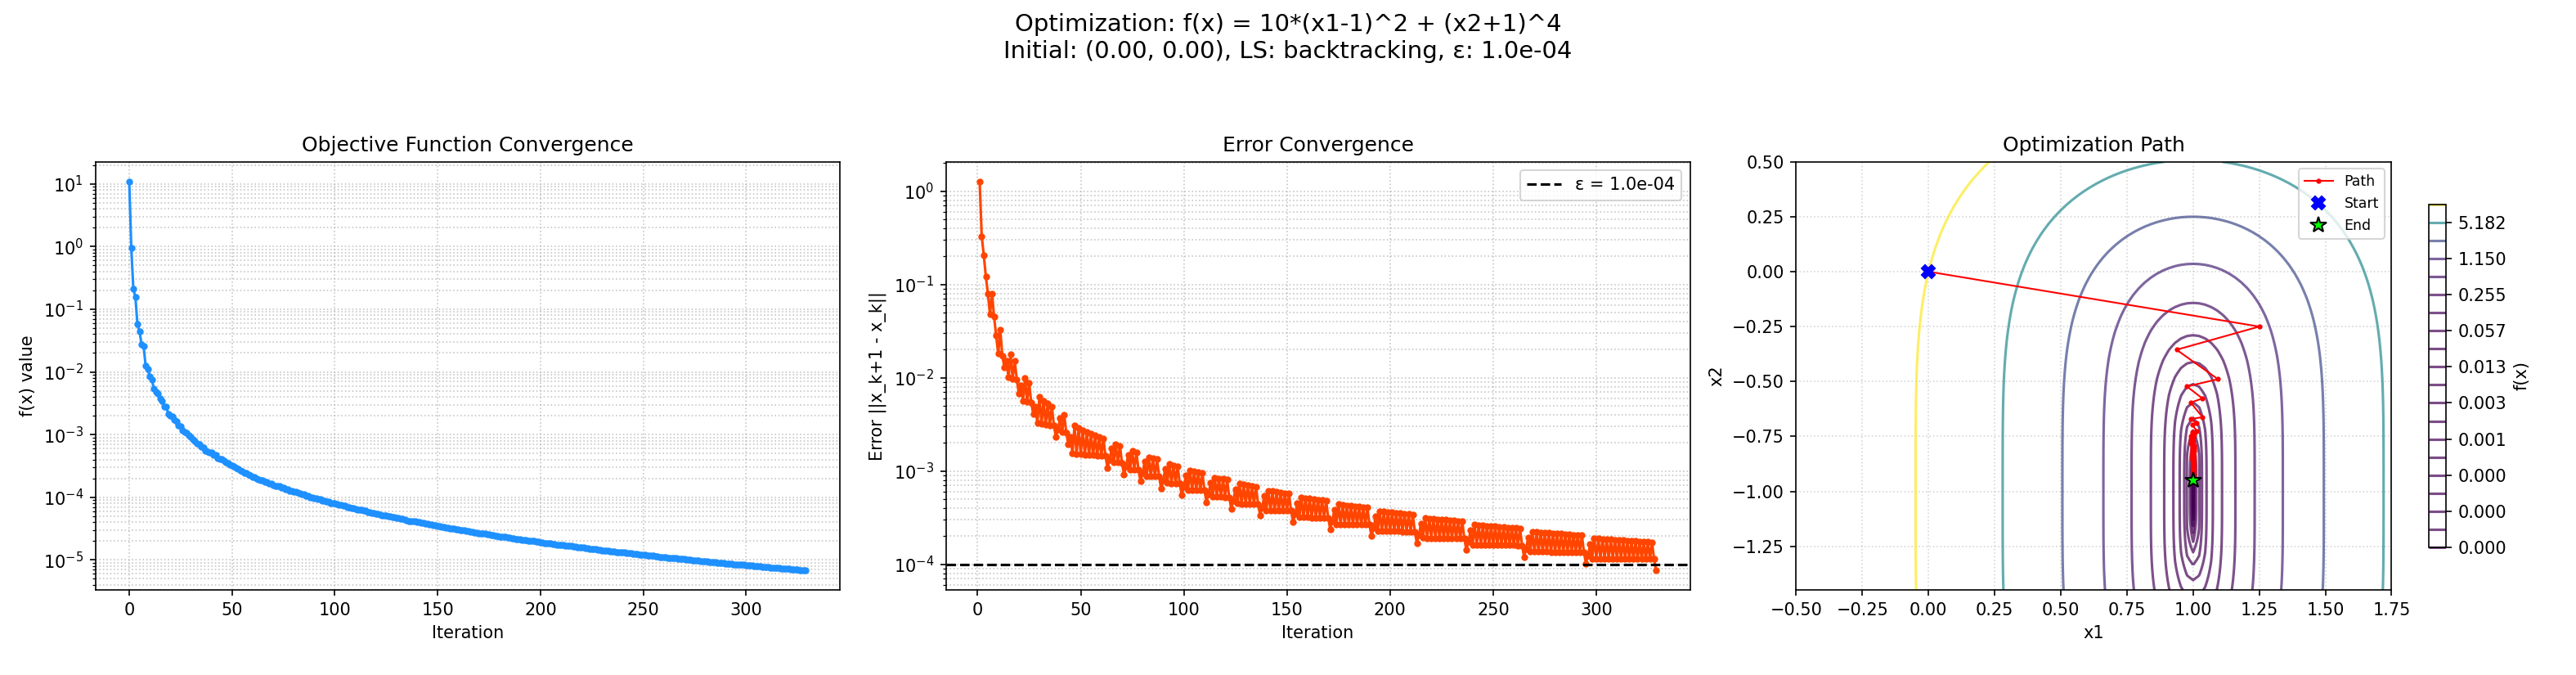
\includegraphics[width=0.9\textwidth]{../fig/opt_F1_x0_0p0_0p0_LS_backtracking_20250524-211744.png}

  \caption{函数1优化过程(回溯线搜索, \(x^{(0)}=(0,0)\), \(\varepsilon=10^{-4}\))}
  \label{fig:f1_results_actual}
\end{figure}

\textbf{分析:} 算法成功收敛,解非常接近理论最优解,目标函数值趋近于0。\(x_2\) 分量未能精确达到-1.0主要受限于 \(\varepsilon\) 及该点附近梯度较小的特性。

\subsubsection{函数2:\(f_2(x_1, x_2) = 100(x_1^2-x_2)^2 + (x_1-1)^2\) (Rosenbrock)}
理论最优解 \(x^*=(1, 1)\),\(f(x^*)=0\)。在达到1000次最大迭代次数后,算法终止。最终解为 \(x^{(1000)} \approx (0.92128, 0.84889)\),目标函数值 \(f(x^{(1000)}) \approx 6.20 \times 10^{-3}\),最终误差 \(\approx 4.25 \times 10^{-4} > \varepsilon\),最终梯度范数 \(\approx 0.1088\)。优化过程如图 \ref{fig:f2_results_actual} 所示。

\begin{figure}[H]
  \centering
  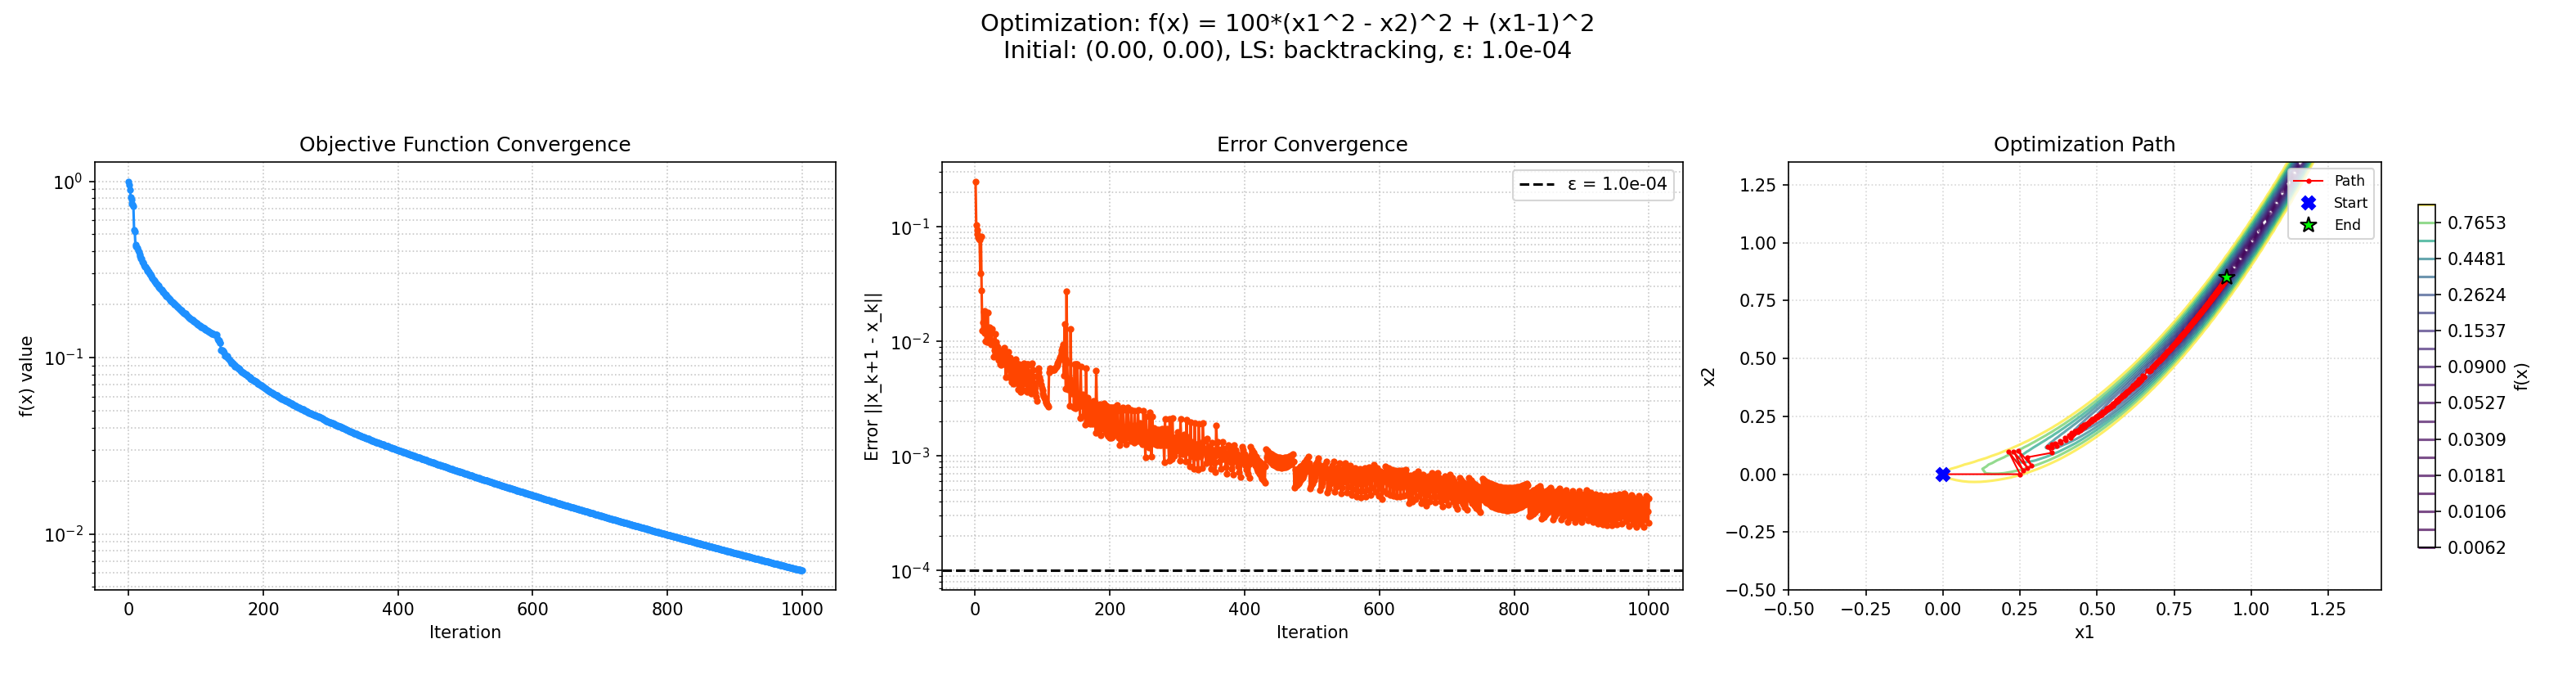
\includegraphics[width=0.9\textwidth]{../fig/opt_F2_x0_0p0_0p0_LS_backtracking_20250524-211825.png}

  \caption{Rosenbrock函数优化过程(回溯线搜索, \(x^{(0)}=(0,0)\), \(\varepsilon=10^{-4}\), MaxIter=1000)}
  \label{fig:f2_results_actual}
\end{figure}

\textbf{分析:} 对于Rosenbrock函数,在1000次迭代内,梯度下降法未能使误差收敛到 \(10^{-4}\) 水平。路径图(如图 \ref{fig:f2_results_actual} 中的等高线部分)会显示典型的沿狭长山谷缓慢前进的“之”字形特点。

\subsubsection{函数3:\(f_3(x_1, x_2) = 100(x_1^2-3x_2)^2 + (x_1-1)^2\)}
理论最优解 \(x^*=(1, 1/3 \approx 0.3333)\),\(f(x^*)=0\)。同样在达到1000次最大迭代次数后,算法终止。最终解为 \(x^{(1000)} \approx (0.93355, 0.29058)\),目标函数值 \(f(x^{(1000)}) \approx 4.42 \times 10^{-3}\),最终误差 \(\approx 2.51 \times 10^{-4} > \varepsilon\),最终梯度范数 \(\approx 0.1286\)。优化过程如图 \ref{fig:f3_results_actual} 所示。

\begin{figure}[H]
  \centering
  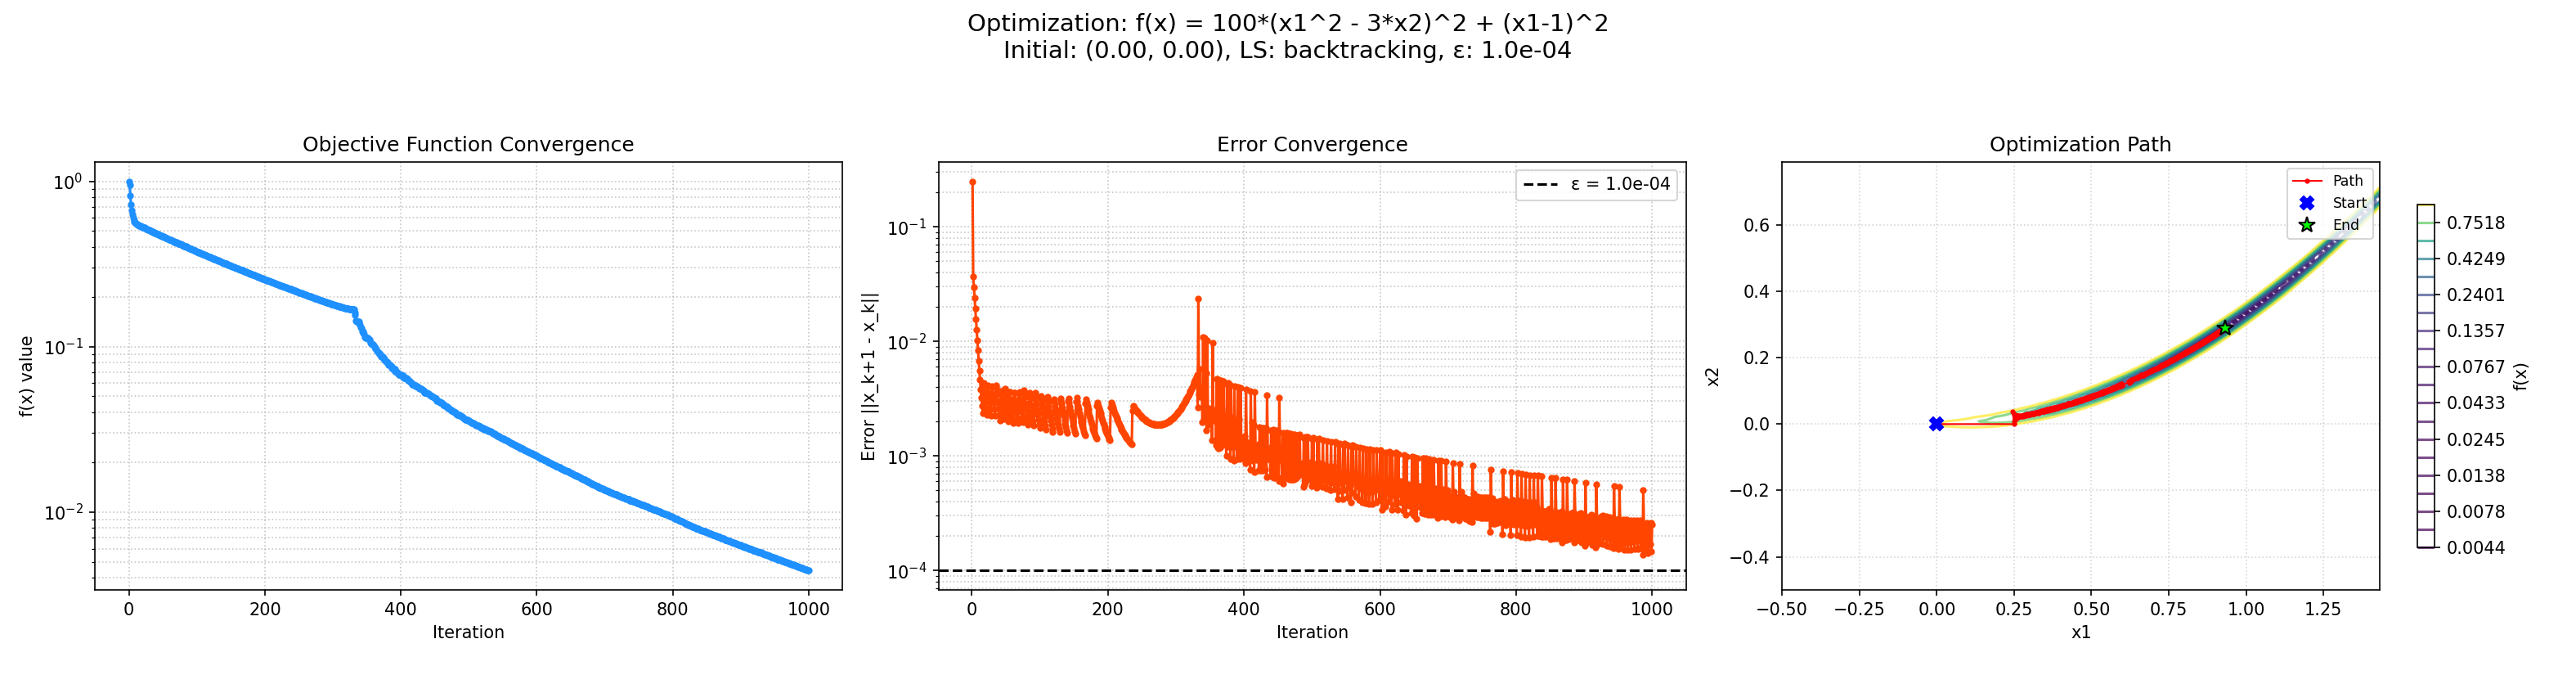
\includegraphics[width=0.9\textwidth]{../fig/opt_F3_x0_0p0_0p0_LS_backtracking_20250524-211846.png}
  
  \caption{函数3优化过程(回溯线搜索, \(x^{(0)}=(0,0)\), \(\varepsilon=10^{-4}\), MaxIter=1000)}
  \label{fig:f3_results_actual}
\end{figure}

\textbf{分析:} 函数3的优化行为与Rosenbrock函数相似,也表现出收敛缓慢的特性。

\subsection{对结果的思考与讨论}
从上述三个实验结果可以看出:
\begin{enumerate}
    \item \textbf{算法有效性与函数依赖性}:梯度下降算法结合回溯线搜索,对结构相对简单的函数(\(f_1\))能有效收敛。对病态特征函数(\(f_2, f_3\)),其收敛速度显著降低。
    \item \textbf{迭代参数的重要性}:初始点、\(\varepsilon\) 和最大迭代次数直接影响优化结果。
    \item \textbf{线搜索策略的角色}:回溯法表现稳健。对于收敛困难的函数,尝试不同(可能更精确的)线搜索方法,有时能改善收敛,但可能增加单次迭代成本。
    \item \textbf{梯度下降法的局限}:本实践清晰展示了梯度下降法作为一阶方法的固有局限性。
    \item \textbf{与CCHP系统优化的关联}:本实践揭示的优化原理和挑战对理解实际CCHP系统经济优化至关重要。
\end{enumerate}

\section{结论与展望}
本实践通过Python编程实现了基于梯度下降法和多种线搜索策略的无约束非线性优化算法。通过对三个典型目标函数的数值实验,验证了算法的有效性,并观察和分析了其收敛特性。主要结论如下:
\begin{enumerate}
    \item 梯度下降法结合有效的线搜索机制,能够稳定地求解无约束优化问题。
    \item 线搜索策略的选择对算法的收敛速度和最终精度有显著影响。
    \item 目标函数的拓扑特性是决定梯度下降法收敛效率的关键外部因素。
    \item 通过编程实践,加深了对迭代优化思想、梯度概念、步长选择重要性以及数值计算中精度与效率权衡的理解。
\end{enumerate}

展望未来,可以在当前工作基础上进行扩展:研究并实现如共轭梯度法、牛顿法、拟牛顿法(BFGS、L-BFGS)等高级梯度方法;将研究扩展到有约束优化问题;并将所学的优化理论与算法应用于更具体的CCHP系统经济调度或设备选型优化模型中。通过这些更深入的学习和实践,可以为解决实际工程中的复杂优化问题打下更坚实的基础。


\appendix
\section{附录:Python代码}
\begin{python}
# cchp_optimize_v3.py
import numpy as np
import matplotlib.pyplot as plt
from scipy.optimize import fsolve, minimize_scalar
import os
import datetime

# --- Global Variables for User Choices (will be set in main) ---
# These are set here to allow plot_optimization_progress to access them
# if they are not passed explicitly, though passing is preferred.
SELECTED_FUNCTION_NUM_GLOBAL = 2
EPSILON_GLOBAL = 1e-4

# --- Objective Functions and Gradients ---
def f1(x):
    x1, x2 = x
    return 10 * (x1 - 1)**2 + (x2 + 1)**4

def grad_f1(x):
    x1, x2 = x
    return np.array([20 * (x1 - 1), 4 * (x2 + 1)**3])

def f2(x):
    x1, x2 = x
    return 100 * (x1**2 - x2)**2 + (x1 - 1)**2

def grad_f2(x):
    x1, x2 = x
    return np.array([400 * x1 * (x1**2 - x2) + 2 * (x1 - 1), -200 * (x1**2 - x2)])

def f3(x):
    x1, x2 = x
    return 100 * (x1**2 - 3*x2)**2 + (x1 - 1)**2

def grad_f3(x):
    x1, x2 = x
    return np.array([400 * x1 * (x1**2 - 3*x2) + 2 * (x1 - 1), -600 * (x1**2 - 3*x2)])

FUNC_MAPPING = {
    1: {"func": f1, "grad": grad_f1, "name": "f(x) = 10*(x1-1)^2 + (x2+1)^4"},
    2: {"func": f2, "grad": grad_f2, "name": "f(x) = 100*(x1^2 - x2)^2 + (x1-1)^2"}, # Rosenbrock
    3: {"func": f3, "grad": grad_f3, "name": "f(x) = 100*(x1^2 - 3*x2)^2 + (x1-1)^2"},
}

# --- Line Search Helper Functions ---
def phi(a, x_k, b_k, objective_func_phi):
    """Helper function for 1D minimization: f(x_k + a*b_k)"""
    return objective_func_phi(x_k + a * b_k)

def phi_prime(a, x_k, b_k, gradient_func_phi):
    """Derivative of phi(a) w.r.t. a: grad_f(x_k + a*b_k) . b_k"""
    x_new = x_k + a * b_k
    grad_at_x_new = gradient_func_phi(x_new)
    return np.dot(grad_at_x_new, b_k)

# --- Robust Line Search Implementations ---
def line_search_fsolve(x_k, b_k, objective_func, gradient_func):
    initial_guess_a = 0.001 
    try:
        a_optimal_roots = fsolve(lambda a_val: phi_prime(a_val, x_k, b_k, gradient_func),
                                 initial_guess_a, xtol=1e-7, maxfev=500) # More precise fsolve
        
        positive_roots = [r for r in np.atleast_1d(a_optimal_roots) if r > 1e-9] 

        if not positive_roots:
            # print(f"Debug (fsolve): No positive root. Roots: {a_optimal_roots}. Fallback.")
            return line_search_backtracking(x_k, b_k, objective_func, gradient_func, alpha_init=0.1)

        best_a = -1
        min_phi_val = phi(0, x_k, b_k, objective_func) # f(x_k)
        
        # Check roots and find the one that minimizes phi(a) the most
        candidate_as = sorted([r for r in positive_roots if r < 50.0]) # Filter large steps
        if not candidate_as: # If all positive roots were too large
             return line_search_backtracking(x_k, b_k, objective_func, gradient_func, alpha_init=0.01)

        for r_val in candidate_as:
            current_phi_val = phi(r_val, x_k, b_k, objective_func)
            if current_phi_val < min_phi_val:
                min_phi_val = current_phi_val
                best_a = r_val
        
        if best_a > 1e-9 : # A valid step was found
             return np.clip(best_a, 1e-9, 20.0) # Clip to reasonable bounds
        else:
            # print(f"Debug (fsolve): No root improved f(x). Fallback.")
            return line_search_backtracking(x_k, b_k, objective_func, gradient_func, alpha_init=0.01)

    except Exception as e:
        # print(f"Error in line_search_fsolve: {e}. Fallback.")
        return line_search_backtracking(x_k, b_k, objective_func, gradient_func, alpha_init=0.01)

def line_search_backtracking(x_k, b_k, objective_func, gradient_func, alpha_init=1.0, beta=0.5, c=1e-4):
    alpha = alpha_init
    f_k = objective_func(x_k)
    # grad_k = gradient_func(x_k) # For Armijo, use grad at x_k
    # slope = np.dot(grad_k, b_k) # b_k is -grad_k, so slope = -||grad_k||^2
    # For simplicity, if b_k is already -grad_k, then grad_k.b_k = -grad_k.grad_k
    slope = np.dot(gradient_func(x_k), b_k)


    if slope > -1e-12 : # Should be significantly negative for descent
        # print(f"Warning (backtracking): Direction b_k (slope: {slope:.2e}) not a strong descent. Using small fixed step.")
        return 1e-5 # Return a very small step

    max_backtrack_iters = 50
    for _ in range(max_backtrack_iters):
        if objective_func(x_k + alpha * b_k) <= f_k + c * alpha * slope:
            return alpha
        alpha *= beta
        if alpha < 1e-10: # Prevent infinitely small steps
            # print("Warning (backtracking): Alpha too small. Using minimal step.")
            return 1e-9 
    # print("Warning (backtracking): Max backtrack iterations reached. Using last alpha.")
    return alpha # Or a very small fixed value if max iters hit

def line_search_minimize_scalar(x_k, b_k, objective_func, gradient_func_for_fallback):
    try:
        res = minimize_scalar(lambda a_val: phi(a_val, x_k, b_k, objective_func),
                              bounds=(0, 20), method='bounded', options={'xatol': 1e-7, 'maxiter':100}) # Wider bounds, more precise
        if res.success and res.x > 1e-9:
            return res.x
        else:
            # print(f"Warning (minimize_scalar): Failed (Success: {res.success}, x: {res.x:.2e}). Fallback.")
            return line_search_backtracking(x_k, b_k, objective_func, gradient_func_for_fallback, alpha_init=0.01)
    except Exception as e:
        # print(f"Error in line_search_minimize_scalar: {e}. Fallback.")
        return line_search_backtracking(x_k, b_k, objective_func, gradient_func_for_fallback, alpha_init=0.01)

# --- Gradient Descent Algorithm ---
def gradient_descent(selected_func_num, x_initial_coords, epsilon_val, max_iters_val, line_search_method_str):
    objective_func = FUNC_MAPPING[selected_func_num]["func"]
    gradient_func = FUNC_MAPPING[selected_func_num]["grad"]
    func_name_str = FUNC_MAPPING[selected_func_num]["name"]

    x_current = np.array(x_initial_coords, dtype=float)
    history = {
        'x_values': [x_current.copy()], 'f_values': [objective_func(x_current)],
        'errors': [], 'gradients_norm': [], 'step_lengths': []
    }
    iterations_completed = 0

    print(f"\n🚀 Optimizing: {func_name_str}")
    print(f"Initial: x0 = {x_current}, f(x0) = {history['f_values'][0]:.6e}")
    print(f"Settings: ε = {epsilon_val:.1e}, MaxIters = {max_iters_val}, LineSearch = {line_search_method_str}")
    print("-" * 95)
    header = f"{'Iter':<5} | {'x1':<13} | {'x2':<13} | {'f(x)':<16} | {'||∇f(x)||':<13} | {'Error':<13} | {'Step (a)':<10}"
    print(header)
    print("-" * 95)

    for k_iter in range(max_iters_val):
        iterations_completed = k_iter + 1
        grad = gradient_func(x_current)
        grad_norm = np.linalg.norm(grad)
        history['gradients_norm'].append(grad_norm)

        b_k = -grad 

        if grad_norm < epsilon_val * 0.001: # More aggressive stop if gradient is tiny
            print(f"\n✅ Gradient norm ({grad_norm:.2e}) is very small. Optimization likely converged.")
            break
        
        if line_search_method_str == 'fsolve':
            a = line_search_fsolve(x_current, b_k, objective_func, gradient_func)
        elif line_search_method_str == 'minimize_scalar':
            a = line_search_minimize_scalar(x_current, b_k, objective_func, gradient_func)
        else: # Default to backtracking
            a = line_search_backtracking(x_current, b_k, objective_func, gradient_func)
        
        history['step_lengths'].append(a)

        if a < 1e-10: # If step length is effectively zero
            print("\n⚠️ Step length 'a' is extremely small. Stopping to prevent stagnation.")
            iterations_completed -=1 
            break

        x_next = x_current + a * b_k
        error = np.linalg.norm(x_next - x_current)

        history['x_values'].append(x_next.copy())
        history['f_values'].append(objective_func(x_next))
        history['errors'].append(error)
        
        # Print progress: first 15, then every 20% of max_iters, or if converged
        if k_iter < 15 or (k_iter + 1) % (max_iters_val // 20 if max_iters_val > 40 else 1) == 0 or error < epsilon_val:
            print(f"{iterations_completed:<5} | {x_next[0]:<13.6f} | {x_next[1]:<13.6f} | {history['f_values'][-1]:<16.6e} | {grad_norm:<13.2e} | {error:<13.6e} | {a:<10.4e}")

        if error < epsilon_val:
            print(f"\n🏁 Convergence achieved at iteration {iterations_completed}: Error < Epsilon.")
            break
        
        x_current = x_next

    print("-" * 95)
    if iterations_completed == max_iters_val and (not history['errors'] or history['errors'][-1] >= epsilon_val):
        print(f"\n⚠️ Maximum iterations ({max_iters_val}) reached. Full convergence may not be achieved.")
    
    final_x = history['x_values'][-1]
    final_f = history['f_values'][-1]
    
    print("\n--- Optimization Summary ---")
    print(f"Function Optimized: {selected_func_num} ({func_name_str})")
    print(f"Initial Point x0: {x_initial_coords}")
    print(f"Epsilon (Accuracy): {epsilon_val:.1e}")
    print(f"Line Search Method: {line_search_method_str}")
    print("-----------------------------")
    print(f"Total Iterations: {iterations_completed}")
    print(f"Optimal x = ({final_x[0]:.8f}, {final_x[1]:.8f})")
    print(f"Optimal f(x) = {final_f:.8e}")
    if history['errors']:
        print(f"Final Error (||Δx||) = {history['errors'][-1]:.8e}")
    if history['gradients_norm']:
         print(f"Final Gradient Norm ||∇f(x)|| = {history['gradients_norm'][-1]:.8e}")

    return history

# --- Plotting and Saving ---
def plot_and_save_results(history, selected_func_num, x_initial_coords, line_search_method_str, epsilon_plot):
    objective_func_plot = FUNC_MAPPING[selected_func_num]["func"]
    func_name_str_plot = FUNC_MAPPING[selected_func_num]["name"]

    if not history['errors'] and len(history['f_values']) <= 1:
        print("\n📉 Not enough data for detailed plotting.")
        return

    num_main_plots = 2 # f(x) vs iter, error vs iter
    x_coords = np.array(history['x_values'])
    plot_contour = x_coords.shape[0] > 1 # Only plot contour if we have iterations
    
    if plot_contour:
        num_main_plots = 3
        
    fig = plt.figure(figsize=(7 * num_main_plots, 5.5)) 

    # Plot 1: Objective Function Value
    ax1 = fig.add_subplot(1, num_main_plots, 1)
    ax1.plot(range(len(history['f_values'])), history['f_values'], marker='.', linestyle='-', color='dodgerblue')
    ax1.set_xlabel("Iteration")
    ax1.set_ylabel("f(x) value")
    ax1.set_title("Objective Function Convergence")
    if any(f_val > 0 for f_val in history['f_values']):
        try:
            ax1.set_yscale('log')
        except ValueError: # Handle cases where values are too small or non-positive for log
            ax1.set_yscale('linear')
    ax1.grid(True, which="both", ls=":", alpha=0.7)

    # Plot 2: Error
    ax2 = fig.add_subplot(1, num_main_plots, 2)
    if history['errors']:
        ax2.plot(range(1, len(history['errors']) + 1), history['errors'], marker='.', linestyle='-', color='orangered')
        ax2.axhline(y=epsilon_plot, color='k', linestyle='--', label=f'ε = {epsilon_plot:.1e}')
        ax2.set_ylabel("Error ||x_k+1 - x_k||")
        ax2.set_title("Error Convergence")
        ax2.set_yscale('log')
        ax2.legend()
    else:
        ax2.text(0.5, 0.5, "No error data", ha='center', va='center')
        ax2.set_title("Error Convergence")
    ax2.set_xlabel("Iteration")
    ax2.grid(True, which="both", ls=":", alpha=0.7)
    
    # Plot 3: Contour plot
    if plot_contour:
        ax3 = fig.add_subplot(1, num_main_plots, 3)
        x1_path = x_coords[:, 0]
        x2_path = x_coords[:, 1]
        
        # Auto-range for contour plot
        x1_min, x1_max = x1_path.min(), x1_path.max()
        x2_min, x2_max = x2_path.min(), x2_path.max()
        x1_range_delta = abs(x1_max - x1_min)
        x2_range_delta = abs(x2_max - x2_min)

        margin_x = max(x1_range_delta * 0.2, 0.5) # Ensure some minimum margin
        margin_y = max(x2_range_delta * 0.2, 0.5)
        
        grid_x1 = np.linspace(x1_min - margin_x, x1_max + margin_x, 100)
        grid_x2 = np.linspace(x2_min - margin_y, x2_max + margin_y, 100)
        
        if np.allclose(grid_x1, grid_x1[0]) or np.allclose(grid_x2, grid_x2[0]):
             ax3.text(0.5,0.5, "Path too small for contour.", ha='center', va='center')
        else:
            X1_grid, X2_grid = np.meshgrid(grid_x1, grid_x2)
            Z_grid = objective_func_plot(np.array([X1_grid, X2_grid]))
            
            levels = 25
            try: # Log levels for functions with large value ranges
                f_vals_positive = [f for f in history['f_values'] if f > 1e-9]
                if f_vals_positive and max(f_vals_positive) / min(f_vals_positive) > 100:
                    levels = np.logspace(np.log10(min(f_vals_positive)), np.log10(max(f_vals_positive)), 20)
            except: pass # Use linear levels if log fails
                
            cp = ax3.contour(X1_grid, X2_grid, Z_grid, levels=levels, cmap='viridis', alpha=0.7)
            fig.colorbar(cp, ax=ax3, label="f(x)", shrink=0.8)
            
            ax3.plot(x1_path, x2_path, 'o-', color='red', markersize=2, linewidth=1, label='Path')
            ax3.plot(x_initial_coords[0], x_initial_coords[1], 'X', color='blue', markersize=8, label='Start')
            ax3.plot(x1_path[-1], x2_path[-1], '*', color='lime', markersize=10, markeredgecolor='black',label='End')
            ax3.set_xlabel("x1")
            ax3.set_ylabel("x2")
            ax3.set_title("Optimization Path")
            ax3.legend(fontsize='small')
            ax3.axis('tight')
            ax3.grid(True, ls=":", alpha=0.5)

    suptitle_text = (f"Optimization: {func_name_str_plot}\n"
                     f"Initial: ({x_initial_coords[0]:.2f}, {x_initial_coords[1]:.2f}), "
                     f"LS: {line_search_method_str}, ε: {epsilon_plot:.1e}")
    fig.suptitle(suptitle_text, fontsize=14)
    plt.tight_layout(rect=[0, 0.02, 1, 0.93]) 

    # Saving the figure
    fig_dir = "fig"
    if not os.path.exists(fig_dir):
        os.makedirs(fig_dir)
        print(f"✅ Created directory: ./{fig_dir}")

    time_stamp = datetime.datetime.now().strftime("%Y%m%d-%H%M%S")
    x0_str_fn = f"{str(x_initial_coords[0]).replace('.', 'p')}_{str(x_initial_coords[1]).replace('.', 'p')}"
    file_name = f"opt_F{selected_func_num}_x0_{x0_str_fn}_LS_{line_search_method_str}_{time_stamp}.png"
    file_path = os.path.join(fig_dir, file_name)

    try:
        plt.savefig(file_path, dpi=150)
        print(f"📊 Figure saved to: {os.path.abspath(file_path)}")
    except Exception as e:
        print(f"❌ Error saving figure: {e}")
    
    plt.show()

# --- Main Execution with User Input ---
if __name__ == "__main__":
    print("--- Gradient Descent Optimization (v3) ---")
    
    while True:
        try:
            prompt = "🎯 Select objective function (1, 2, or 3, default 2):\n"
            for i, data in FUNC_MAPPING.items():
                prompt += f"   {i}: {data['name']}\n"
            prompt += "Choice: "
            SELECTED_FUNCTION_NUM_GLOBAL = int(input(prompt) or "2")
            if SELECTED_FUNCTION_NUM_GLOBAL in FUNC_MAPPING:
                break
            print("Invalid selection. Please enter 1, 2, or 3.")
        except ValueError: print("Invalid input. Please enter a number.")

    while True:
        try:
            x0_input_str = input("📍 Enter initial point x0 as 'x1,x2' (e.g., 0,0 or -1.2,1, default 0,0): ") or "0,0"
            user_x_initial = [float(x.strip()) for x in x0_input_str.split(',')]
            if len(user_x_initial) == 2: break
            print("Please enter two comma-separated values for x1 and x2.")
        except ValueError: print("Invalid format. Use 'x1,x2' (e.g., 0.0,0.0).")
    
    while True:
        try:
            EPSILON_GLOBAL = float(input(f"🔍 Enter convergence epsilon ε (e.g., 1e-4, default {1e-4:.1e}): ") or f"{1e-4:.1e}")
            if EPSILON_GLOBAL > 0: break
            print("Epsilon must be positive.")
        except ValueError: print("Invalid number for epsilon.")

    while True:
        try:
            user_max_iterations = int(input(f"🔄 Enter maximum iterations (e.g., 1000, default 1000): ") or "1000")
            if user_max_iterations > 0: break
            print("Maximum iterations must be positive.")
        except ValueError: print("Invalid integer for maximum iterations.")

    while True:
        user_line_search_method = input(
            "🌊 Select line search: 'fsolve', 'backtracking', 'minimize_scalar' (default 'backtracking'): "
        ).lower() or "backtracking"
        if user_line_search_method in ['fsolve', 'backtracking', 'minimize_scalar']: break
        print("Invalid method. Choose from the list.")

    # Call the optimization
    hist = gradient_descent(SELECTED_FUNCTION_NUM_GLOBAL, user_x_initial, EPSILON_GLOBAL, 
                              user_max_iterations, user_line_search_method)
    
    # Plot and save results
    plot_and_save_results(hist, SELECTED_FUNCTION_NUM_GLOBAL, user_x_initial, 
                          user_line_search_method, EPSILON_GLOBAL)

    print("\n--- Expected Optimal Solutions (Approximate) ---")
    expected = {
        1: "x ≈ (1.0, -1.0), f(x) ≈ 0",
        2: "x ≈ (1.0, 1.0), f(x) ≈ 0 (Rosenbrock)",
        3: "x ≈ (1.0, 0.333), f(x) ≈ 0"
    }
    print(f"For Function {SELECTED_FUNCTION_NUM_GLOBAL}: {expected.get(SELECTED_FUNCTION_NUM_GLOBAL, 'N/A')}")
    print("\n✨ Optimization complete.")
\end{python}

\end{document}